\documentclass{beamer}
\usepackage[english]{babel} 
\usepackage[latin1]{inputenc} 
\usepackage{amsthm}
\usepackage{dsfont}
\usepackage{xcolor}
\usepackage{multimedia}
 
\title{Preprocessing and Classification \\ of ERD/ERS Signals}
%\subtitle{Untertitel}
\author{Florian Eichin \\ Advisor: Andreas Meinel}
\institute{Freiburg University}
\date{July 17, 2018}

\usetheme{metropolis}

\selectlanguage{english}
\setbeamercolor{background canvas}{bg=white}

 
\begin{document}

\maketitle

\begin{frame}
	\frametitle{Contents of this Talk}
	\begin{itemize}
	\item[1.] How do we measure brain activity?
	\item[2.] Oscillatory Analysis
	\item[3.] Noise, Dimension, Localization
	\item[4.] Spatial Filters
	\begin{itemize}
	\item Laplace Filters
	\item Common Spatial Patterns (CSP)
	\end{itemize}
	\item[5.] Classifying ERD/ERS
	\end{itemize}
\end{frame}

\begin{frame}
\frametitle{Goal/Motivation for this talk}
Via brain activity: Classify (imagined) left/right hand movement \\
	\begin{center}
	\includegraphics[scale=0.15]{motivation1.png}
	\end{center}
	{\bf How can we achieve this?}
\end{frame}

\section{How do we measure brain activity?}

\begin{frame}
\frametitle{Which technology do we use?}
	\begin{itemize}
	\item Many ways to measure brain activity:
	\begin{itemize}
		\item fMRI, fNIR
		\item EEG, MEG, ECoG
	\end{itemize}
	\item Invasive or non-invasive?
	\item Trade-off: time and spatial resolution, costs, mobility
	\item {\bf In this talk: electromagnetic activity via EEG}
	\end{itemize}
	\centering
	\includegraphics[scale=0.24]{kappe.jpg}
	{\tiny [Wolpaw, 2011]}
\end{frame}

\begin{frame}
	\frametitle{Representation of EEG-Signals}
	\centering
	\only<1>{\includegraphics[scale=0.18]{headandwaves1.png}}
	\only<2>{\includegraphics[scale=0.18]{headandwaves2.png}}
	\only<3>{\includegraphics[scale=0.18]{headandwaves4.png}}
	\begin{itemize}
	\item \only<1-3>{ Let $t, d, C\in \mathds{N}$}
	\item \only<1-3>{A {\bf \textcolor{red}{sample}} is a vector ${\bf \textcolor{red}{x}} \in \mathds{R}^{C}$}
	\item \only<2-3>{$\textcolor{blue}{X} = \textcolor{blue}{(}\textcolor{red}{{\bf x}^{(t)}} \ \textcolor{red}{{\bf x}^{(t+1)}} \ ... \ \textcolor{red}{{\bf x}^{(t+d)}}\textcolor{blue}{)} \in \mathds{R}^{Cxd}$ is called an {\bf \textcolor{blue}{epoch}}}
	\item \only<3>{We will use labeled epochs for training our classifier}
	\end{itemize}
\end{frame}

\begin{frame}
\frametitle{Next step to our goal}
	Via brain activity: Classify (imagined) left/right hand movement
	\begin{center}
	
	\includegraphics[scale=0.15]{motivation2.png}
	\end{center}
	{\bf What features of measured brain activity are useful?}
\end{frame}


\section{Oscillatory Analysis: Some Background }

\begin{frame}
\frametitle{Pyramidal Cells - Generators of EEG}
	\begin{itemize}
	\item Largest contributor to electromagnetic activity
	\item Aligned orthogonally to the cortex surface
	\item Electromagnetic fields add up whenever we have co-aligned, co-activated activity
	\item[$\rightarrow$] {\bf Only large scale, synchronous activity picked up by EEG}
	\end{itemize}
	\centering
	% \only<1>{\includegraphics[scale=0.25]{pyramidal_aligned.jpg}	\\}
	\only<1>{\includegraphics[scale=0.33]{pyramidal_alignedpm.png}	\\}
	{\tiny [Aarhuus University, 2004]}
\end{frame}

\begin{frame}
\frametitle{Idle Oscillations - What we assume}
\begin{itemize}
	\item Inactive populations of neurons enter an {\bf idle state}
	\item They fire synchronously at characteristic frequencies
	\begin{itemize}
		\item[] e.g. $\alpha$- / $\mu$-rhythms: 8-15 Hz, found in visual / motor cortex
	\end{itemize}
	\item Can be observed on frequency spectrum:
	\end{itemize}
	\centering
	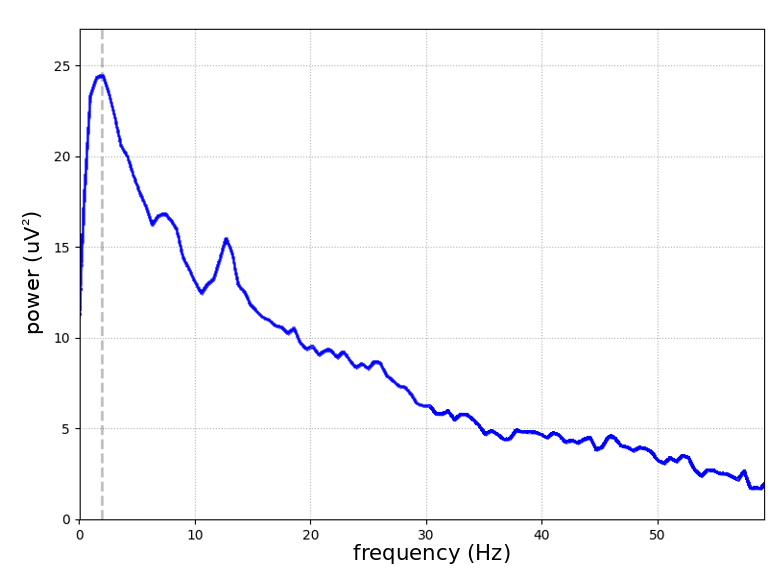
\includegraphics[scale=0.25]{psd.png}
\end{frame}

\begin{frame}
\frametitle{Event Related (De)Synchronizations}
	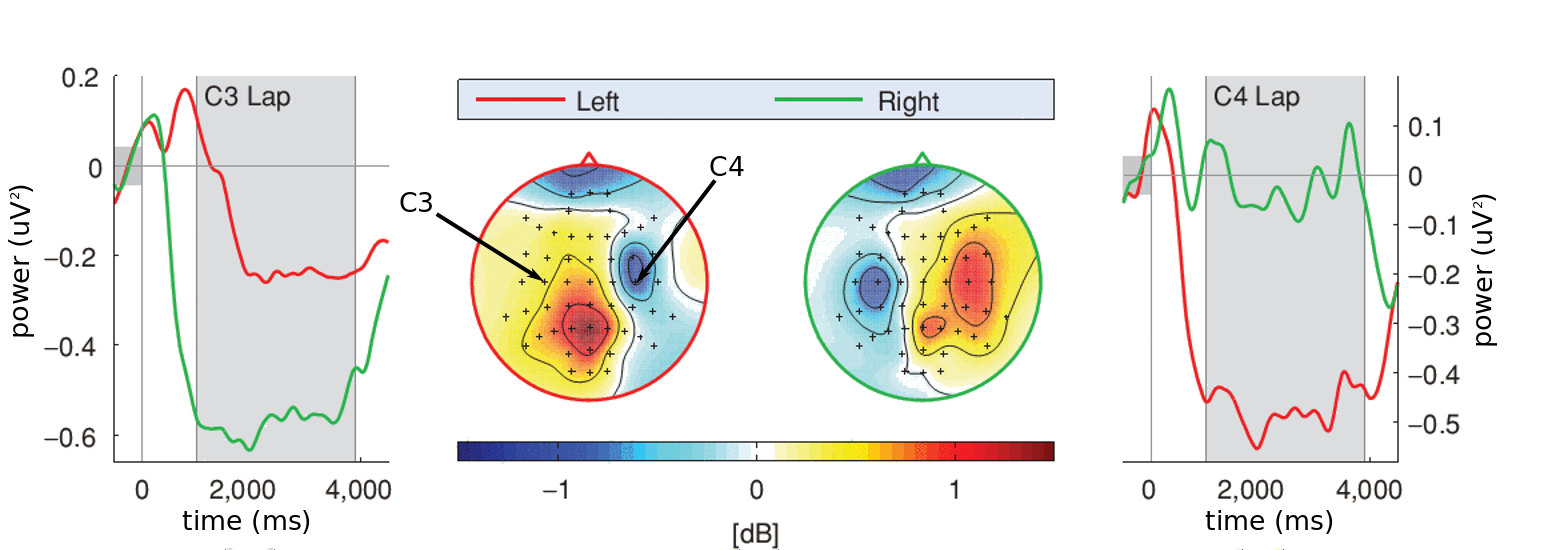
\includegraphics[scale=0.21]{spectralrarr.png}
	{\tiny [Blankertz, 2008]}
	\begin{itemize}
	\item increase of power = Event Related Synchronization ({\bf ERS})
	\item decrease of power = Event Related Desynchronization ({\bf ERD})
	\item Parts of the brain are linked to certain tasks
	\item[$\rightarrow$] Local ERD/ERS will help discriminating left and right hand
	\end{itemize}
\end{frame}

\begin{frame}
\frametitle{We're still looking at Problems}
	Via brain activity: classify (imagined) left/right hand movement \\
	\begin{center}
	\includegraphics[scale=0.15]{motivation3.png}
	\end{center}
	{\bf Why don't we just look for local ERD/ERS?}
\end{frame}


\section{Noise, Dimension and Localization: What are the challenges?}

\begin{frame}
\frametitle{Noise and Dimension}
\begin{itemize}
 	\item Raw EEG-data has low signal-to-noise ratio
 	\item Also high dimensionality (up to 128 channels)
 	\item[$\rightarrow$]{\bf We need a lot of training data}
\end{itemize}
\centering
	{\tiny [University of Nebraska, 2013]}
 	\includegraphics[scale=0.27]{cap.jpg}
\end{frame}

\begin{frame}
\frametitle{Localization of ERD/ERS activity}
\centering
	\begin{itemize}
	\item Brain processes have high subject-to-subject variation
	\item Even with the same subject we will have high session-to-session variation
	\item[$\rightarrow$]{\bf New session/subject: Localize relevant ERD/ERS again}
	\end{itemize}
\end{frame}

\begin{frame}
\frametitle{We need Preprocessing}
	Via brain activity: Classify (imagined) left/right hand movement
	\begin{center}
	\includegraphics[scale=0.12]{motivation4.png}
	\end{center}
	{\bf How can we improve signal-to-noise ratio, decrease dimensionality and deal with localization?}
\end{frame}



\section{Simple solution: Laplace Filters}


\begin{frame}
	\frametitle{What is a Spatial Filter?}   
	\begin{itemize}
	\item $C$ the \textcolor{blue}{number of channels} \\
	\item A {\bf spatial filter} is a vector ${\bf w} \in \mathds{R}^{\textcolor{blue}{C}}$
	\item For a sample ${\bf x} \in \mathds{R}^C$ the filtered sample is
	\begin{equation}
		\tilde{x} = {\bf w}^T \cdot {\bf x} \in \mathds{R}
	\end{equation}
	\end{itemize}
\end{frame}

\begin{frame}
	\begin{center}
	\frametitle{Laplace Filters}
	\centering
	\only<1>{\includegraphics[scale=0.265]{lfilter1.png}}
	\only<2>{\includegraphics[scale=0.265]{lfilter2.png}}
	\only<3-5>{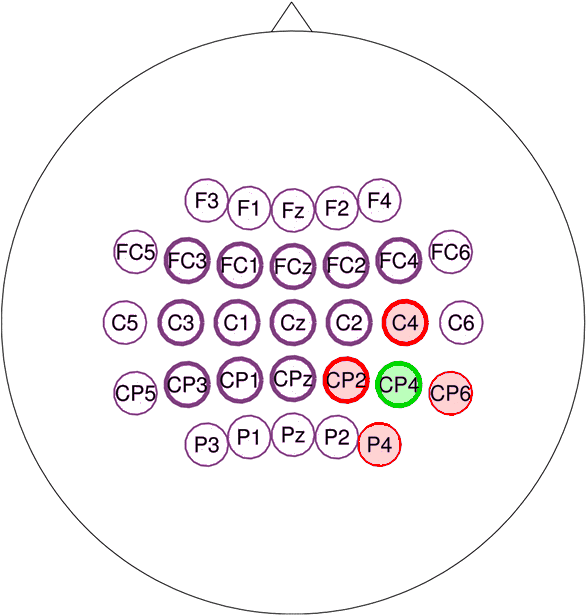
\includegraphics[scale=0.265]{lfilter3.png}}
	\end{center}
	\only<1-5>{${\bf x} = (x_{F3}, ..., x_{P4})^T$ \\}
	\only<4-5>{${\bf w} = (0, ..., 0, \textcolor{red}{-\frac{1}{4}}, \textcolor{red}{-\frac{1}{4}}, \textcolor{green}{1}, \textcolor{red}{-\frac{1}{4}}, \textcolor{red}{-\frac{1}{4}})^T$ \\}
	\only<5>{$\tilde{x} = {\bf w}^T \cdot {\bf x} =  \textcolor{red}{-\frac{1}{4} \cdot (x_{C4} + x_{CP2} + x_{CP6} + x_{P4})} + \textcolor{green}{x_{CP4}}$}
\end{frame}

\begin{frame}
\frametitle{What can be achieved?}
\includegraphics[scale=0.36]{spectralp.png}
\includegraphics[scale=0.26]{rsquared.png}
{\tiny [Blankertz, 2008]}
\begin{itemize}
 	\item Slight peak in $\mu$-range at around 12 Hz
 	\item[$\rightarrow$] $r^2$-score indicates: already useful discriminability
\end{itemize}
\end{frame}

\begin{frame}
\frametitle{Are Laplace Filters what we searched for?}

	\begin{center}
    \begin{tabular}{ | l | l | l | p{3cm} |}
    \hline
   	Solution & SNR & Dimensionality & Localization \\ \hline
    Laplace Filters & \textcolor{orange}{Somewhat} & \textcolor{green}{Yes} & \textcolor{red}{By hand} \\ \hline
    \end{tabular}
\end{center}

	{\bf How can we (further) improve signal/noise ratio, decrease dimensionality and deal with localization?}

\end{frame}

\begin{frame}
\frametitle{Are Laplace Filters what we searched for?}

	\begin{center}
   \includegraphics[scale=0.3]{learn.png}
\end{center}

	{\bf How can we (further) improve signal/noise ratio, decrease dimensionality and deal with localization?}

\end{frame}

\section{A data-driven approach: \\ Common Spatial Patterns (CSP)}

\begin{frame}
	\frametitle{Common Spatial Patterns (CSP)}
	\begin{itemize}
	\item Learn filters from sample epochs $X_i \in \mathds{R}^{CxD}$ for class \textcolor{blue}{L} and \textcolor{olive}{R}
	\item Variance in EEG channels estimates average power of signal
	\item Idea: {\bf Contrast variance} between the two classes
	\end{itemize}
	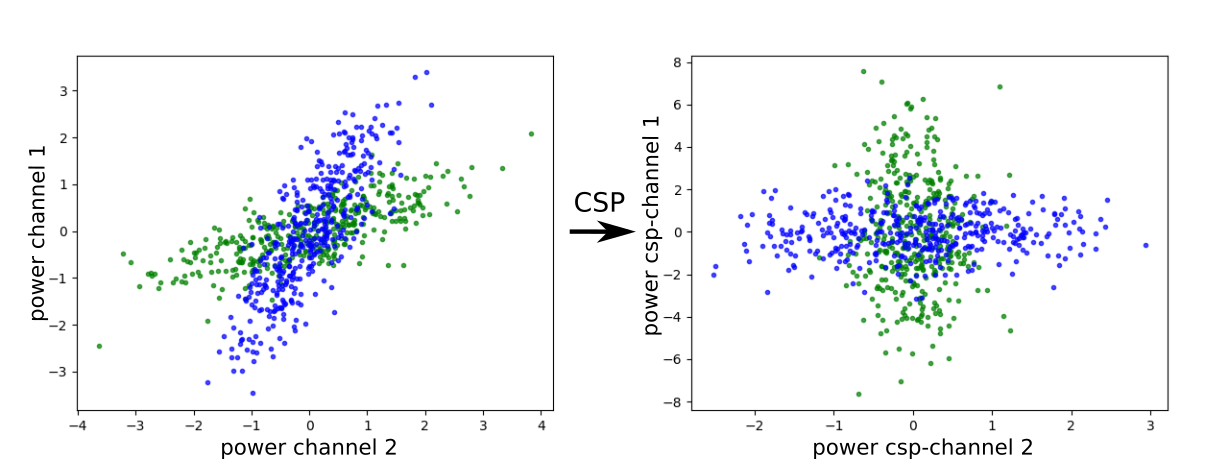
\includegraphics[scale=0.28]{scattered.png}
	%\includegraphics[scale=0.325]{scatter_csp.png}
\end{frame}

\begin{frame}
	\frametitle{CSP Step I - Covariance Estimation}
	\begin{itemize}
	\item Let $X_1, ..., X_k \in \mathds{R}^{CxD}$ be the sample epochs for class $h$
	\item Then we estimate the {\bf covariance matrix} by
	\begin{equation}
		\Sigma_h = \frac{1}{k} \sum_{i=1}^{k}X_i X_i^T
	\end{equation}
	\end{itemize} 
\end{frame}

\begin{frame}
	\frametitle{CSP Step II - Optimization Problem}
	\begin{itemize}
	\item Let $\Sigma_{L}, \Sigma_{R} \in \mathds{R}^{CxC}$ be the covariance matrix for class L / R
	\item Subsequently find orthogonal vectors ${\bf w}_i$ that satisfy
	\begin{equation}
		{\bf w}_i = \underset{{\bf w} \in \mathds{R}^{C}}{argmax} \  \frac{{\bf w}^T \Sigma_{L} {\bf w}}{{\bf w}^T \Sigma_{R} {\bf w}}
	\end{equation}
	\only<2>{\item $W = ({\bf w}_1 \ ... \ {\bf w}_N)^T$ projects data to a space, where the first coordinate has the highest (lowest) variance for class L (R)
	\item[$\rightarrow$] in application: only keep first and last couple of vectors}
	\end{itemize}
\end{frame}

\begin{frame}
\frametitle{Analytical Solution for the Optimization Problem}
	This optimization problem can be solved with Lagrange Multipliers:
	\begin{columns}
	\begin{column}{0.9\textwidth}
	\begin{block}
	\only<2-7>{$\rightarrow$ {\bf maximize} \textcolor{blue}{${\bf w}^T \Sigma_{L} {\bf w} $ }{\bf w.r.t.} \textcolor{purple}{$ {\bf w}^T \Sigma_{R} {\bf w} = c$\\}}
	\begin{block}
	\only<3-7>{$L(\lambda, {\bf w}) =  \textcolor{blue}{{\bf w}^T \Sigma_{L} {\bf w}} - \lambda ( \textcolor{purple}{{\bf w}^T \Sigma_{R} {\bf w} - c})$ \\} 
	\begin{block}
	\only<4-7>{$\frac{\partial}{\partial {\bf w}} L(\lambda, {\bf w}) = 2 \Sigma_{L} {\bf w} - \lambda 2 \Sigma_{R} {\bf w}$} 
	\only<5>{$\textcolor{brown}{\overset{!}{=}0}$}	
	\only<6-7>{$\overset{!}{=}0$}
	\begin{block}
	\only<6-7>{$\Leftrightarrow$ \ $\Sigma_{L} {\bf w} = \lambda \Sigma_{R} {\bf w}$}
	\end{block} \end{block} \end{block} \end{block}		
	\end{column}
	\end{columns}
	%\begin{block}
	\only<7>{\begin{itemize}
	\item Which is a {\bf generalized eigenvalue problem} \\
	\item Eigenvectors ${\bf w}_1, ..., {\bf w}_n$ with eigenvalues $\lambda_1 > \lambda_2 >...> \lambda_n$ yield $W = ({\bf w}_1 \ ... \ {\bf w}_n)^T$
	\end{itemize}}
	%\end{block}
\end{frame}

\begin{frame}
\frametitle{CSP in Action}
	\centering
	\only<1>{\includegraphics[scale=0.29]{video_start_csp.png}
	\tiny [Tangermann, 2018]}
	\only<2>{\movie[autostart]{\includegraphics[scale=0.29]{video_start_csp.png}}{csp_video.avi}
	\tiny [Tangermann, 2018]}
\end{frame}

\begin{frame}
\frametitle{Evaluation: Even better results}
	\begin{itemize}
	\item $\alpha$- and $\mu$-bands are more prominent after filtering
	\item $r^2$-score: Good discriminanility in CSP-channel
	\end{itemize}
	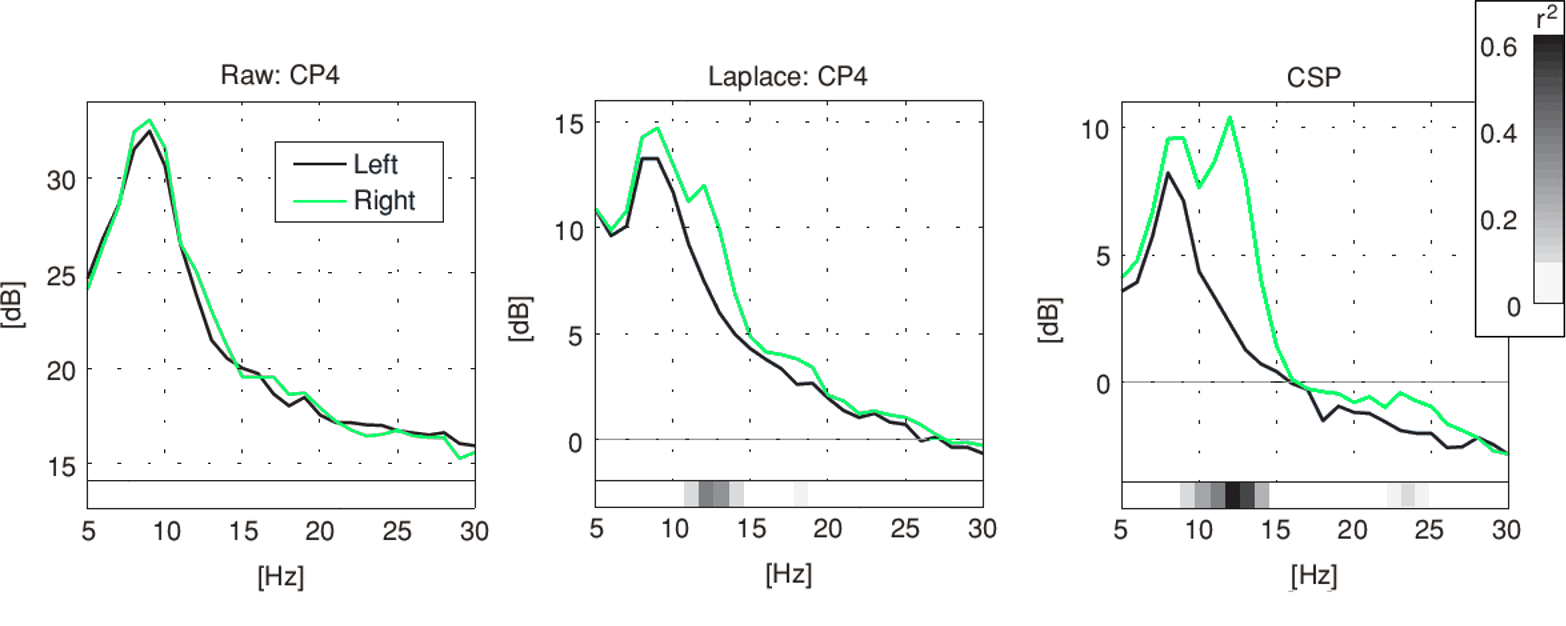
\includegraphics[scale=0.20]{spectracsplp.png}
	{\tiny [Blankertz, 2008]}
	%\includegraphics[scale=0.18]{rsquared.png}
\end{frame}

\begin{frame}
\frametitle{Are CSP-filters what we searched for?}
	\begin{center}
    \begin{tabular}{ | l | l | l | p{3cm} |}
    \hline
   	Solution & SNR & Dimensionality & Localization \\ \hline
    Laplace Filters & \textcolor{orange}{Somewhat} & \textcolor{green}{Yes} & \textcolor{red}{By hand} \\ \hline
    CSP & \textcolor{green}{Yes} & \textcolor{green}{Yes} & \textcolor{green}{Yes} \\ \hline
    \end{tabular}
\end{center}
	\begin{itemize}
	\item easy to use and implement
	\item analytical solution
	\item low runtime (linear mapping)
	\item on the other hand:
	\begin{itemize}
	\item hyperparameters (length, time point of epochs ...)
	\item supervised: need for labeled data
	\end{itemize}
	\end{itemize}

\end{frame}

\section{Final Step: Classification}

\begin{frame}
\frametitle{Let's put it together! - Intuition}

\begin{itemize}
	\item[1.]\only<1-4>{ Fetch labeled epochs from participant}
	\item[2.]\only<2-4>{ Compute CSP-filters on bandpassed (e.g. 8-15 Hz) epochs}
	\item[3.]\only<3-4>{ Use the outer CSP-channels (highest contrast in power!)}
	\item[4.]\only<4>{ Train classifier on average power of  CSP-channels of epoch}
\end{itemize}
\centering
	\only<1>{\includegraphics[scale=0.9]{class10.png}}
	\only<2>{\includegraphics[scale=0.9]{class6.png}}
	\only<3>{\includegraphics[scale=0.9]{class9.png}}
	\only<4>{\includegraphics[scale=0.9]{class7.png}}
\end{frame}

\begin{frame}
\frametitle{Conclusion - Did we achieve our goal?}
\begin{center}
\only<1>{\includegraphics[scale=0.15]{motivation1.png}}
\only<2>{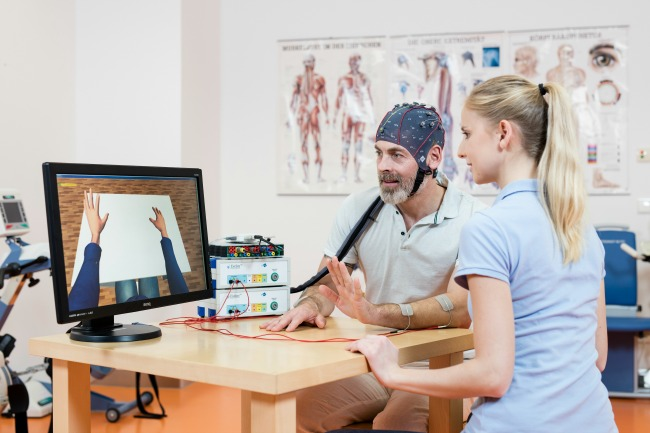
\includegraphics[scale=0.3]{rehab.JPG}}
\only<3>{\includegraphics[scale=0.12]{game.jpg}}
\end{center}
\begin{itemize}
\item In [1] this approach was used with average accuracy of 90\% 
\item[$\rightarrow$] {\bf this could be useful for a lot of tasks already}
\end{itemize}
\end{frame}


\begin{frame}
\frametitle{Sources}
\begin{itemize}
	\item[[1]] Blankertz B, Tomioka R, Lemm S, Kawanabe M, Mueller KR, Optimizing Spatial Filters for Robust EEG Single-Trial Analysis. IEEE Signal Process Mag, 25(1):41-56, 2008.
	\item[[2]] Wolpaw, Brain-Computer Interfaces: principles and practice. Oxford Univ. Press, 2011.
	\item[[3]] mne$\-$tools.github.io/dev/auto$\_$examples/decoding/ \\ plot$\_$decoding$\_$csp$\_$eeg.html
	\item[[4]] Schalk, G McFarland, DJ Hinterberger T, Birbaumer N, Wolpaw JR, BCI2000: A General-Purpose Brain-Computer Interface (BCI) System. IEEE TBME 51(6):1034-1043, 2004
	\item[[5]] Introduction to Modern Brain-Computer Interface Design - Christian A. Kothe Swartz Center for Computational Neuroscience, University of California San Diego
\end{itemize}
\end{frame}

\begin{frame}
	\frametitle{Filters and Patterns}
	
	$W$ consists of filters, the rows of $A = W^{-1}$ are called patterns. \\
	\centering
	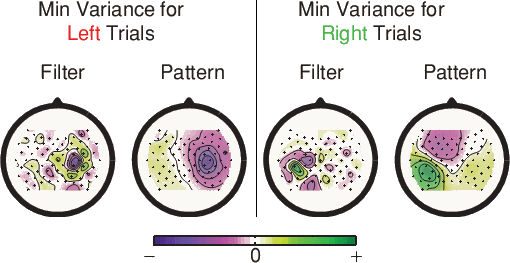
\includegraphics[scale=0.4]{topos.png}
\end{frame}

\begin{frame}
\frametitle{Relation to Principal Component Analysis}
	CSP is a supervised generalization of PCA for two classes. \\
	If class {\bf R} is is uncorrelated, CSP yields the same filter matrix as PCA for class {\bf L}.
	
	\begin{proof}
	Let $\Sigma_{L}$ and $\Sigma_{R}$ be the covariance matrices for class L and R. \\
	Then $\Sigma_{R} = I$ and we have 
	\begin{equation}
	w_i = \underset{w \in \mathds{R}^{N}}{argmax} \frac{w^T \Sigma_{L} w}{w^T \Sigma_{R} w} = \underset{w \in \mathds{R}^{n}}{argmax} \frac{w^T \Sigma_{L} w}{w^T w}
	\end{equation}
	which is the optimization criterion for PCA.
	\end{proof}		
\end{frame}

\begin{frame}
\frametitle{Idle Oscillations - Video}
\centering
	\only<1>{\includegraphics[scale=0.22]{video_start.png}
	\tiny [Backyard Brains, 2014]}
	\only<2>{\movie[autostart]{\includegraphics[scale=0.22]{video_start.png}}{alpha.mp4}
	\tiny [Backyard Brains, 2014]}
\end{frame}

\begin{frame}
\frametitle{So what could this classifier look like?}
We train and use the following classifier:
\begin{equation}
	f(X,
	 {\bf w}_1, ..., {\bf w}_J, 
	 \beta_0, ..., \beta_J) =
	 \sum_{j=1}^{J} 
	 \only<5>{\textcolor{blue}{\beta_j}} \only<1-4, 6>{\beta_j} 
     \only<4>{\textcolor{blue}{\log}}\only<1-3, 5-6>{\log}(
	 	\only<3>{\textcolor{blue}{{\bf w}^T_j }} \only<1-2, 4-6>{{\bf w}^T_j}
	 	\only<1,3-6>{XX^T}\only<2>{\textcolor{blue}{X X^T}} 
	 	\only<3>{\textcolor{blue}{{\bf w}_j }} \only<1-2, 4-6>{{\bf w}_j}
	 ) 
	 + \only<5>{\textcolor{blue}{\beta_0}} \only<1-4, 6>{\beta_0}
\end{equation}
	\begin{itemize}
	\item \only<2-6>{ for EEG-epoch $X \in \mathds{R}^{CxD}$, estimate \only<2>{\textcolor{blue}{covariance}}\only<3-6>{covariance} ($\sim$power)}
	\item \only<3-6>{ filter the signal with \only<3>{\textcolor{blue}{CSP-filters}}\only<4-5>{CSP-filters} ${\bf w}_1, ..., {\bf w}_J$}
	\item \only<4-6>{take the \only<4>{\textcolor{blue}{logarithm}}\only<5-6>{logarithm} of the power of the projected signal}
	\item \only<5-6>{\only<5>{\textcolor{blue}{$\beta_0, ..., \beta_J$}}\only<6>{$\beta_0, ..., \beta_J$} are the \only<5>{\textcolor{blue}{bias and weights}} \only<6>{bias and weights}, that need to be trained on sample epochs (e.g. via LDA)}
	\item \only<6>{sign of the weighted sum is a prediction of labels (L/R labels need to be exchanged with $+1/-1$)}
	\end{itemize}
\end{frame}

\end{document}